\documentclass{article}
\usepackage{ctex}

\title{数字逻辑与计算机组成\\ {\small 实验 6: 单周期 CPU 设计与测试
}}
\author{王卫东\quad 221900332}
\date{\zhtoday}

\usepackage{hyperref}
\usepackage{algorithm}
\usepackage{algorithmicx}
\usepackage{algpseudocode}
\usepackage{float}  
\usepackage{lipsum}
\usepackage{color, xcolor}
\usepackage{listings}
\usepackage{dirtree}
\usepackage{ulem}
\usepackage{graphicx}
\usepackage{amsmath}
\usepackage{amssymb}
\usepackage{amsfonts}
\usepackage{xcolor}
\usepackage{tikz}
\usepackage{multirow}
\usepackage{zhnumber} % change section number to chinese
\usepackage{listings}



\renewcommand\thesection{\zhnum{section}}
\renewcommand\thesubsection{\arabic{subsection}}
\usetikzlibrary{arrows,shapes,chains}

\begin{document}
    \maketitle

    \section{实验目的}

    \begin{enumerate}
        \item 掌握 RV32I 控制器的设计方法。
        \item 掌握单周期 CPU 中的时序设计。
        \item 掌握 RISC-V 汇编语言程序的基本设计方法。
        \item 理解汇编语言程序与机器语言代码之间的对应关系。
    \end{enumerate}
    \section{实验环境}

    Logisim:https://github.com/Logisim-Ita/Logisim \\
    RISC-V 模拟器工具 RARS:https://github.com/thethirdone/rars

    \section{实验内容}
    
    \subsection{控制器设计实验}

    \subsubsection{整体方案设计}
    \begin{figure}[H]
    \centering
    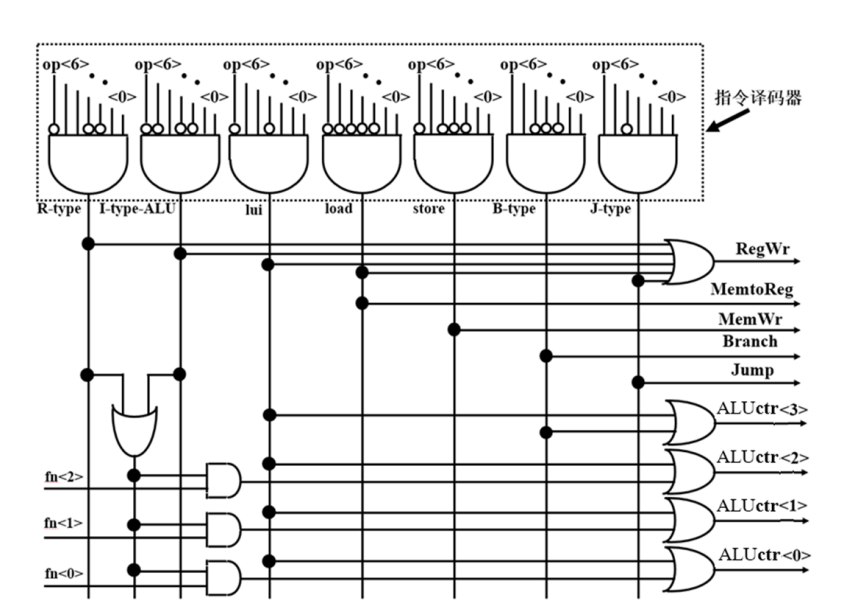
\includegraphics[width=0.4\textwidth]{1.1.png}
    \caption{控制器整体方案设计}
    \end{figure}

    \subsubsection{引脚作用}
    \begin{table}[H]
    \centering
    \begin{tabular}{|c|c|}
        \hline
        opcode  & 指令代码中的操作码 \\ \hline
        funct3  & 指令代码中的功能码 \\ \hline
        funct7  & 指令代码中的功能码 \\ \hline
        ExtOp  & 指令代码中的扩展操作码 \\ \hline
        RegWr  & 寄存器写使能 \\ \hline
        ALUASrc  & ALU 第一个操作数选择信号 \\ \hline
        ALUBSrc  & ALU 第二个操作数选择信号 \\ \hline
        ALUctr  & ALU 控制信号 \\ \hline
        MemWr  & 存储器写使能 \\ \hline
        MentoReg  & 存储器读数据到寄存器使能 \\ \hline
        Branch  & 分支使能 \\ \hline
        MemOp  & 存储器读写选择信号 \\ \hline
        halt  & 停机信号 \\ \hline
        U-lui等 & 7位指令code用一位标志位表示 \\ \hline
    \end{tabular}
    \caption{控制器引脚作用}
    \end{table}
    RV32I 指令控制信号列表见数逻实验报告6指南,此处只截取了一部分。
    \begin{figure}[H]
    \centering
    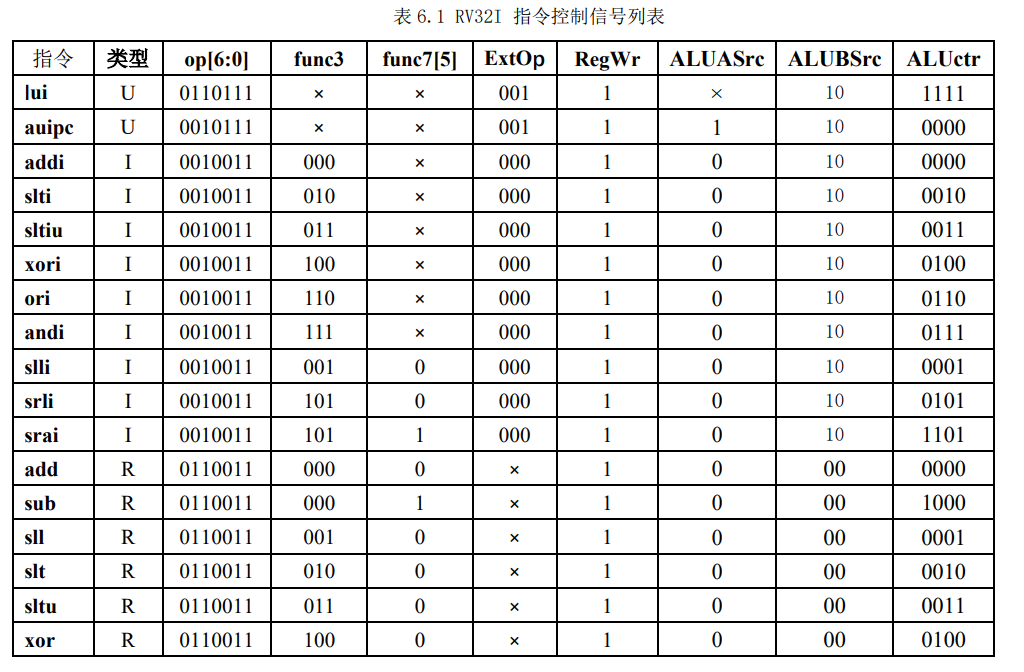
\includegraphics[width=0.4\textwidth]{1.2.png}
    \caption{RV32I 指令控制信号}
    \end{figure}

    \subsubsection{原理图和电路图}
    原理图同整体方案设计图。

    \begin{figure}[H]
    \centering
    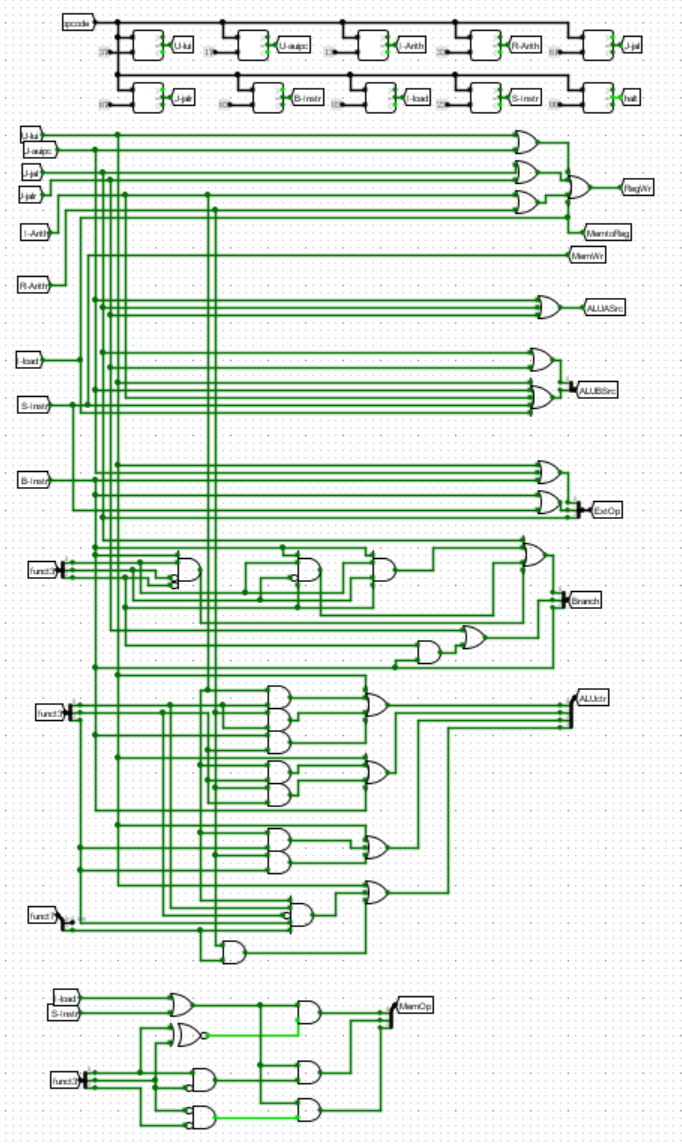
\includegraphics[width=0.8\textwidth]{1.4.2.png}
    \caption{控制器电路图}
    \end{figure}

    \subsubsection{仿真测试图}
    \begin{figure}[H]
    \centering
    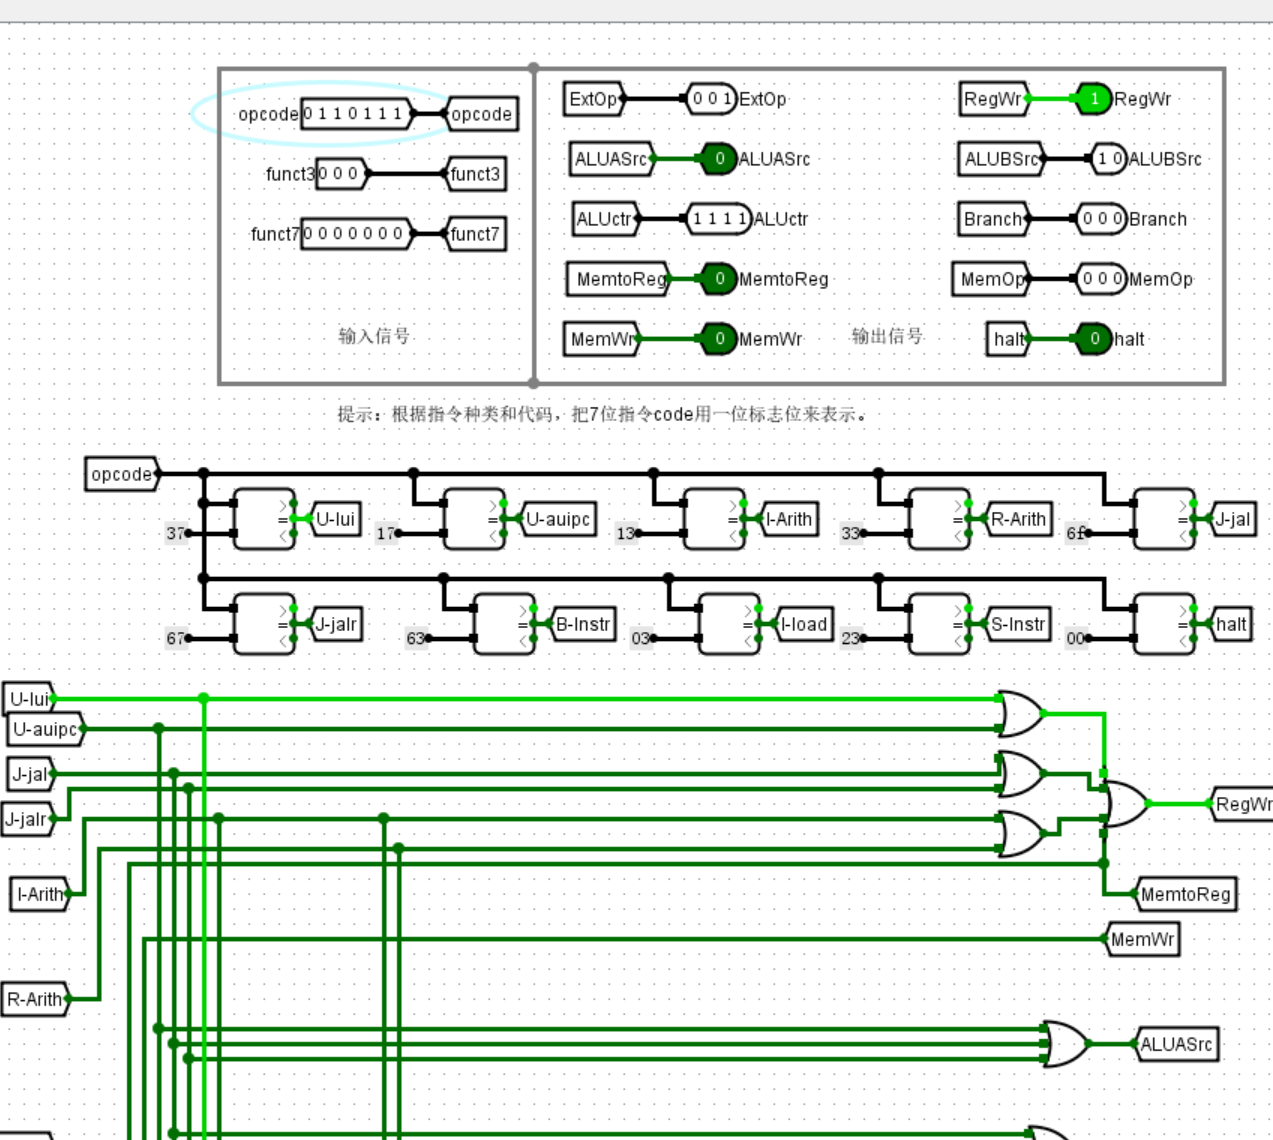
\includegraphics[width=0.4\textwidth]{1.5.1.png}
    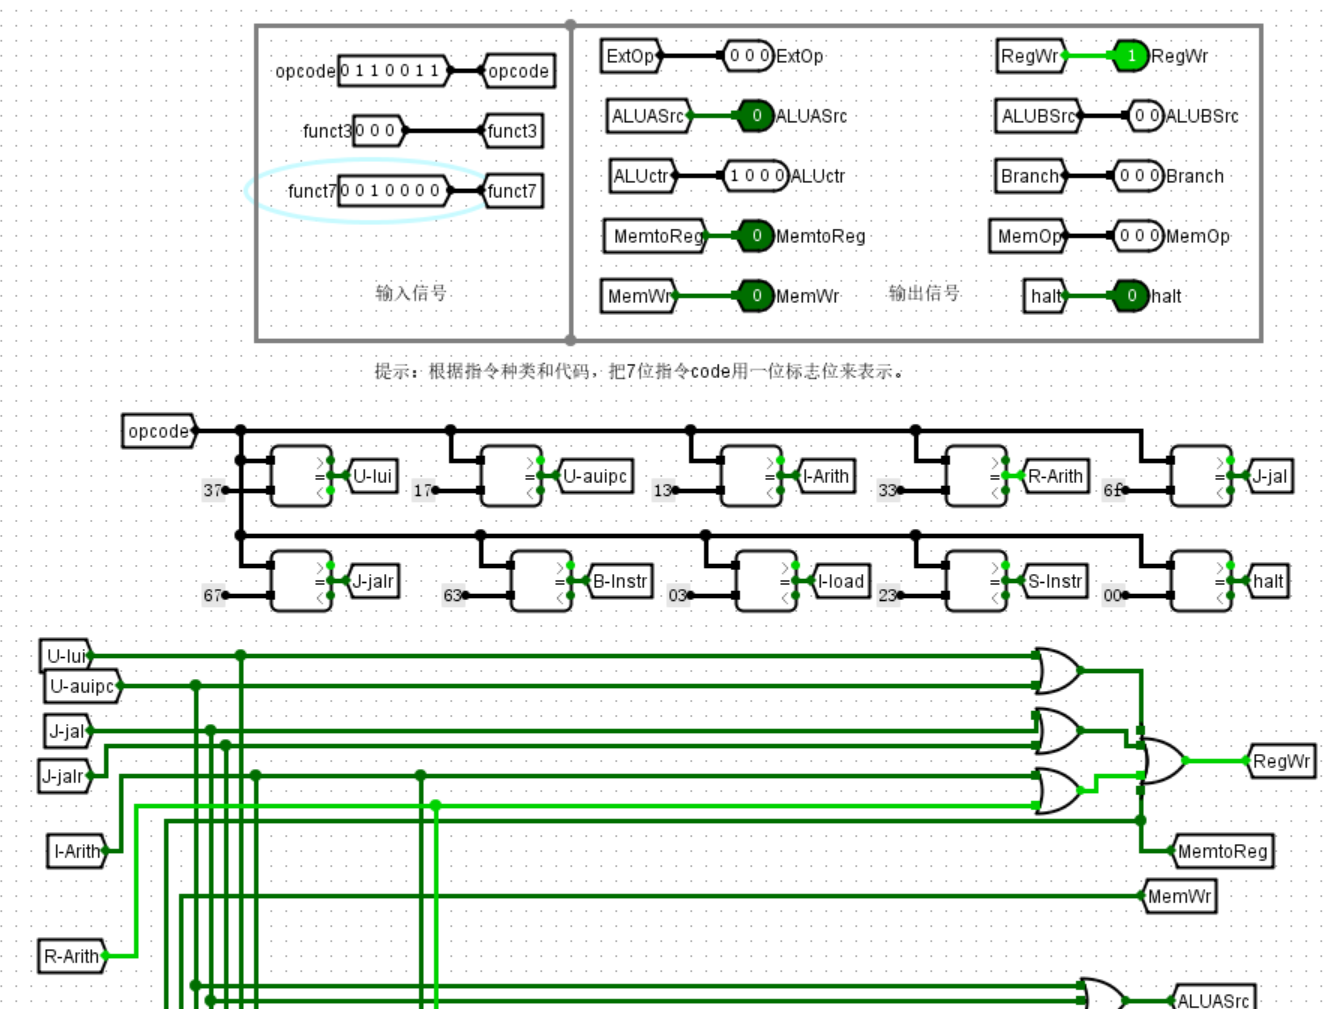
\includegraphics[width=0.4\textwidth]{1.5.2.png}
    
    \caption{控制器仿真测试图}
    \end{figure}

    \begin{figure}[H]
    \centering
    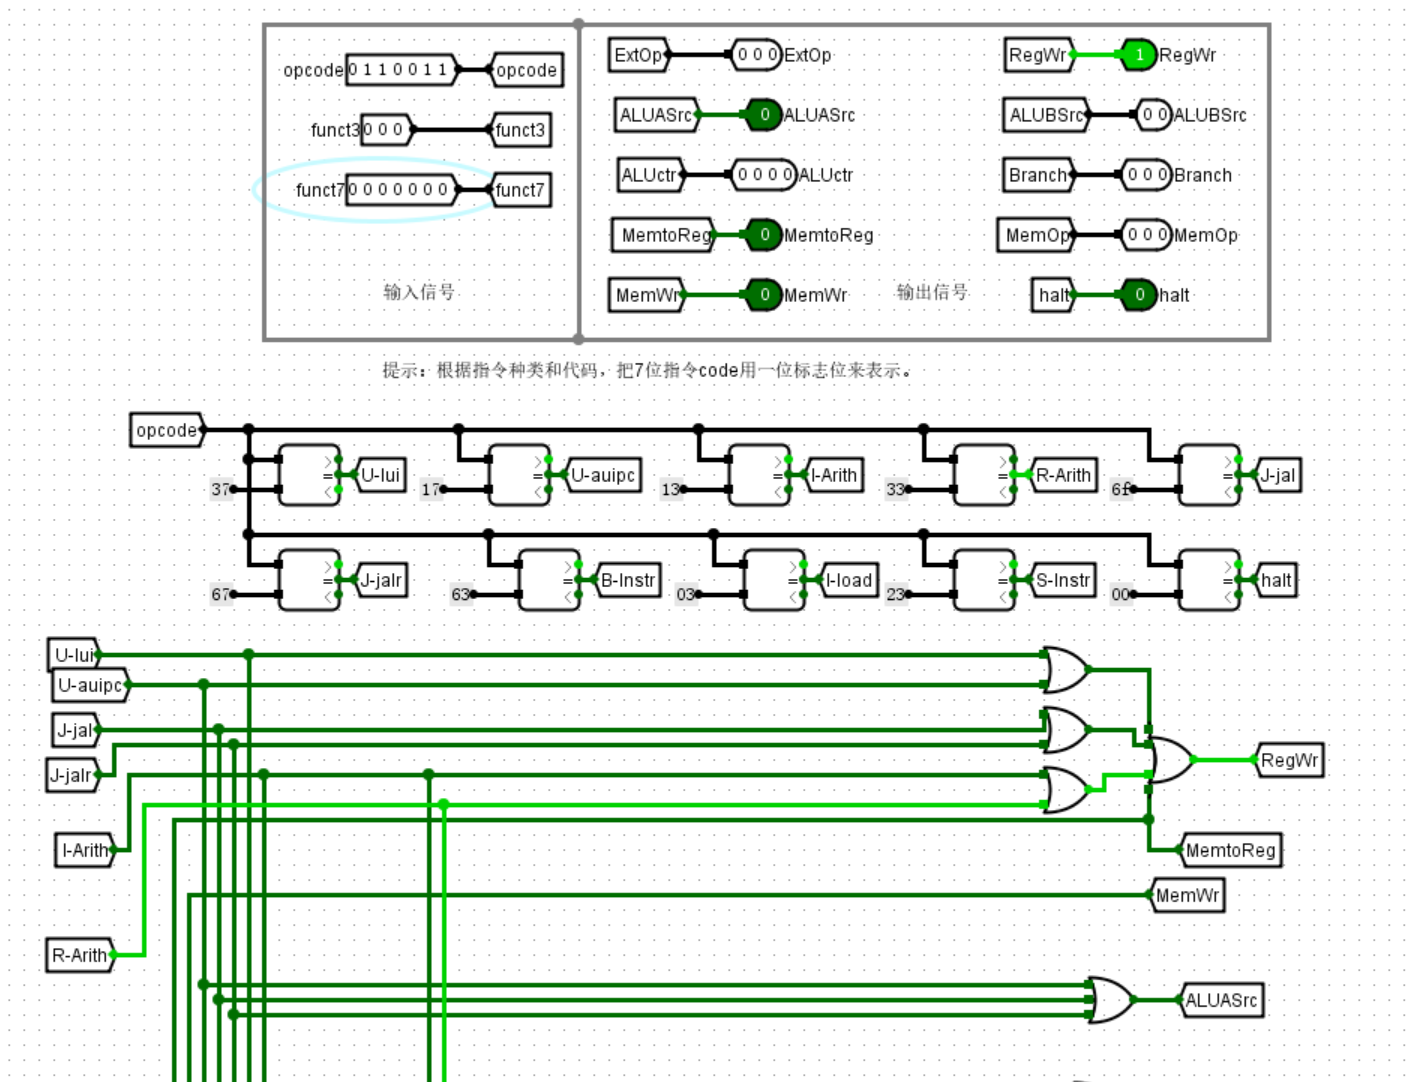
\includegraphics[width=0.4\textwidth]{1.5.3.png}  
    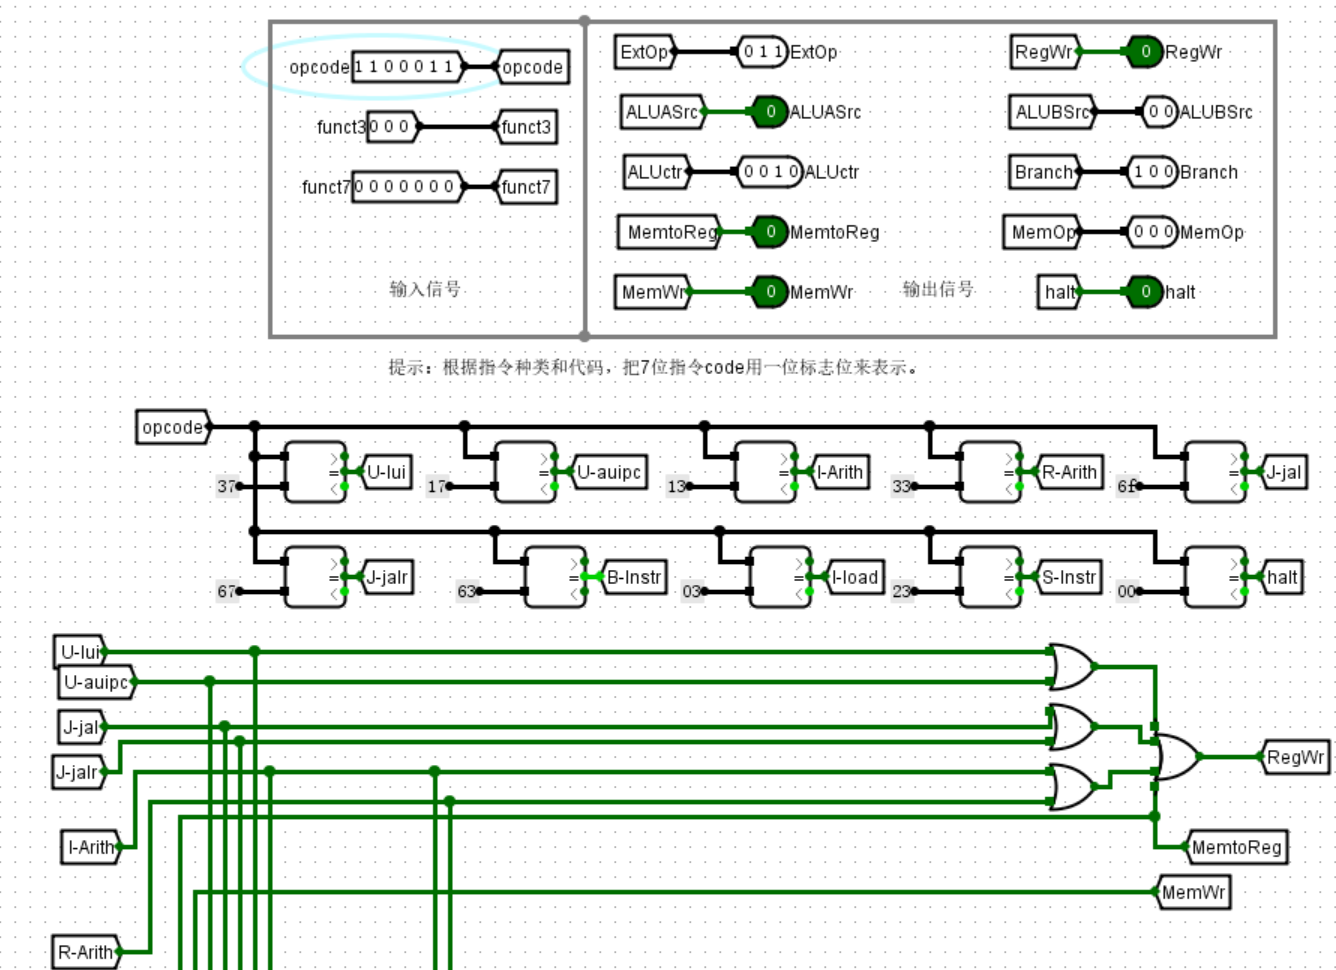
\includegraphics[width=0.4\textwidth]{1.5.4.png}
    \caption{控制器仿真测试图}
    \end{figure}
    
    \begin{itemize}
        \item 图 1 为lui指令,opcode=0110111,funct3=000,funct7=0000000,ExtOp=001,RegWr=1,ALUASrc=0,ALUBSrc=10,ALUctr=1111,MemWr=0,MentoReg=0,Branch=0,MemOp=0,halt=0,符合预期。
        \item 图 2 为sub指令,opcode=0110011,funct3=000,funct7=0010000,ExtOp=000,RegWr=1,ALUASrc=0,ALUBSrc=00,ALUctr=1000,MemWr=0,MentoReg=0,Branch=0,MemOp=0,halt=0,符合预期。
        \item 图 3 为add指令,opcode=0110011,funct3=000,funct7=0000000,ExtOp=000,RegWr=1,ALUASrc=0,ALUBSrc=00,ALUctr=0000,MemWr=0,MentoReg=0,Branch=0,MemOp=0,halt=0,符合预期。
        \item 图 4 为beq指令,opcode=1100011,funct3=000,funct7=0000000,ExtOp=011,RegWr=0,ALUASrc=0,ALUBSrc=00,ALUctr=0010,MemWr=0,MentoReg=0,Branch=100,MemOp=0,halt=0,符合预期。
    \end{itemize}
    
    

    \subsubsection{错误现象及分析}
    在完成实验的过程中,没有遇到任何错误。

    \subsection{单周期 CPU 设计实验}

    \subsubsection{整体方案设计}
    在单周期 CPU 中,每条的指令都需要在一个时钟周期内完成。本次实验中,以时钟下降沿为每个时钟周期的开始,写入操作在时钟下降沿时同步实现,而读取操作,则是异步实现,只要输入有效地址后,立即输出对应数据。同时需要考虑的时序信号,有复位信号 Reset、片选信号 Sel、中止信号 halt 等。\par
    整体上只需要加入控制器,对实验5中的DataPath的引脚略作修改即可。

    \subsubsection{顶层模块设计}
    在前期的实验中已经完成全部模块的设计,在实验 3 中实现了寄存器堆模块,实验 4 中实现了 ALU 模块,实验 5 中实现了数据存储器、取指令部件和数据通路模块,本次实验完成了控制器模块。

    \subsubsection{引脚作用}
    \begin{table}[H]
    \centering
    \begin{tabular}{|c|c|}
        \hline
        clk   & 时钟信号 \\ \hline
        Init Addr & 初始化地址 \\ \hline
        Reset & 复位信号 \\ \hline
        Halt & 中止信号 \\ \hline
        Halt0 & 判断程序执行周期终止信号 \\ \hline
    \end{tabular}
    \caption{单周期 CPU引脚作用}
    \end{table}

    \subsubsection{原理图和电路图}
    \begin{figure}[H]
        \centering
        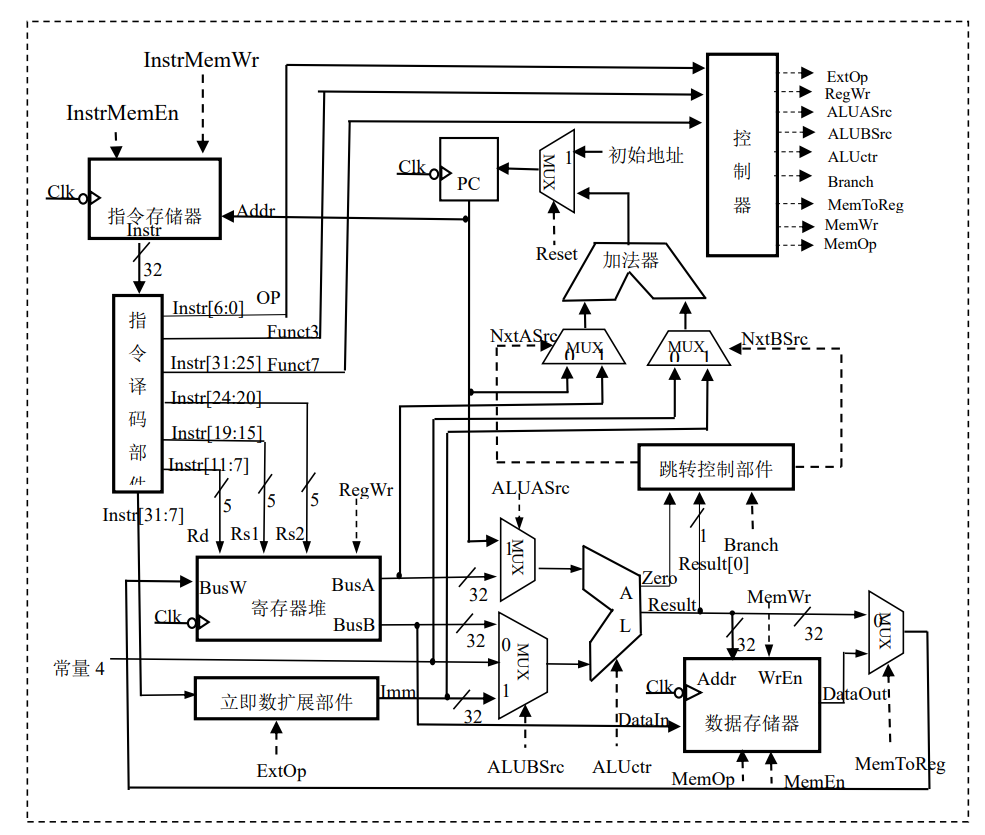
\includegraphics[width=0.8\textwidth]{2.4.1.png}
        \caption{单周期 CPU原理图}
        \end{figure}

    \begin{figure}[H]
    \centering
    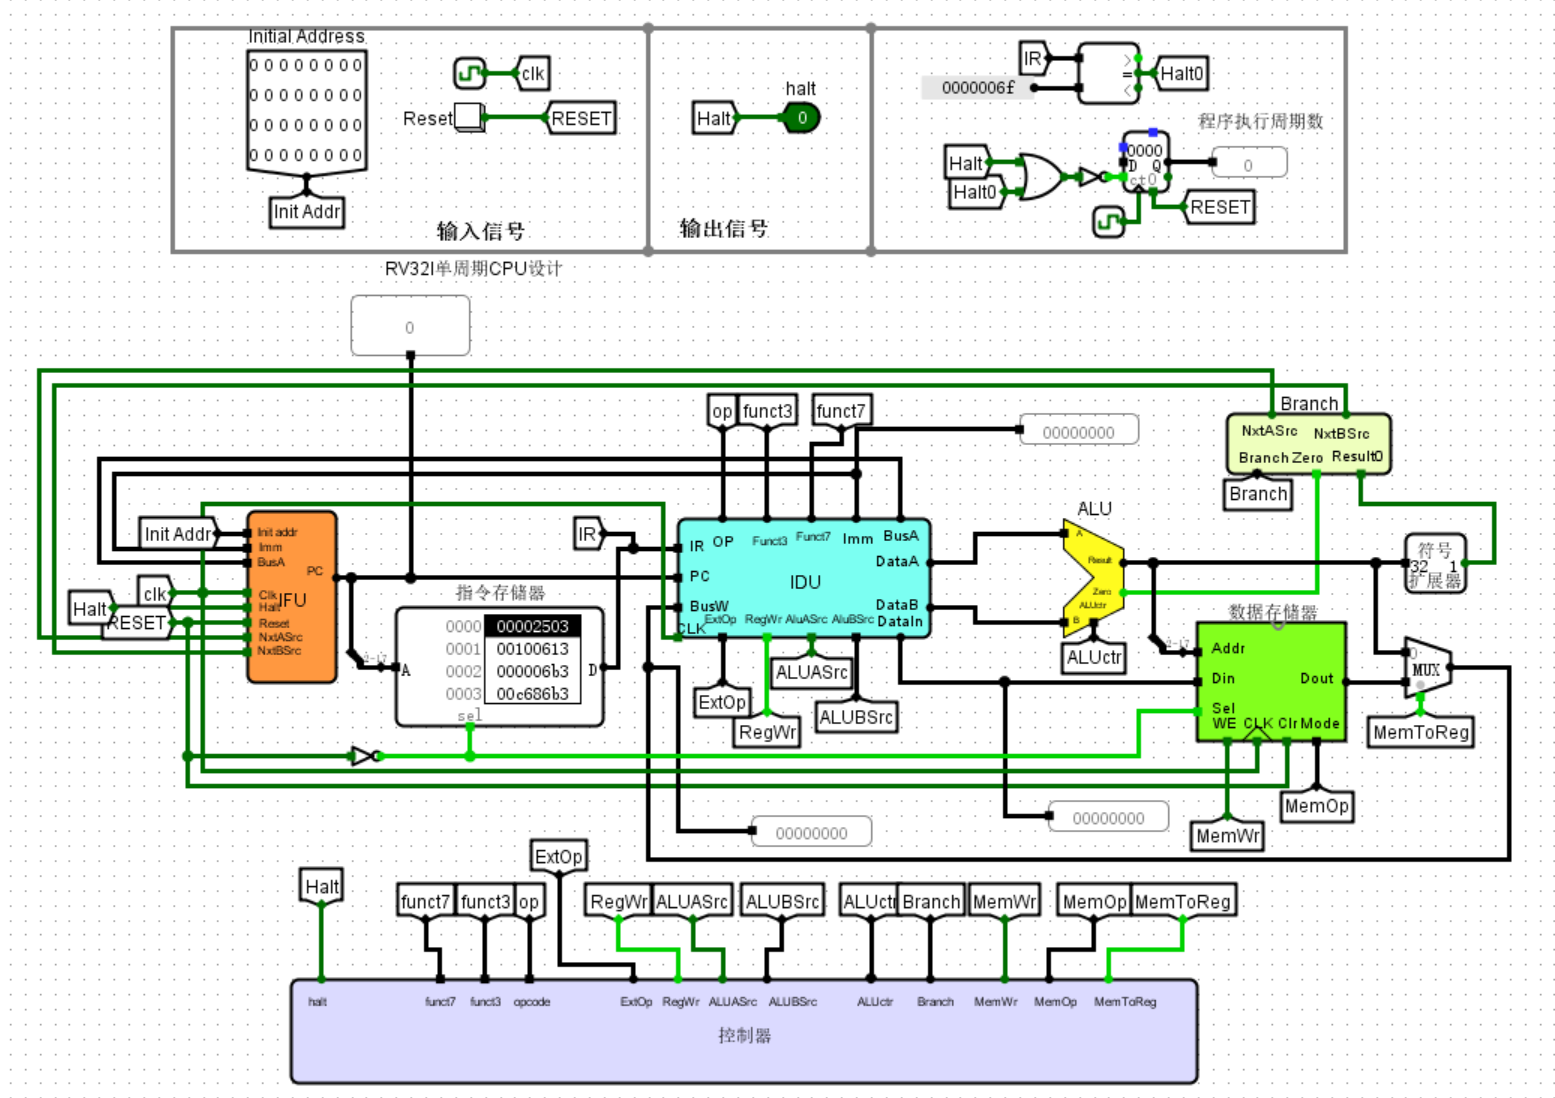
\includegraphics[width=0.8\textwidth]{2.4.2.png}
    \caption{单周期 CPU电路图}
    \end{figure}

    \subsubsection{仿真测试图}
    仿真测试见下三个验收实验。

   

    \subsubsection{错误现象及分析}
    在完成实验的过程中,经常遇到Regfile红线的情况,经检查是Regfile中线路重叠的问题,将其解决后,仿真测试通过。

    \subsection{用累加和程序验证 CPU 设计}
    首先,将计算累加和的 RV32I 汇编语言程序在 RARS 中调试通过,汇编成机器代码并导出。然后将机器代码载入到 CPU 的指令存储器部件中。设置参数 n,启动时钟信号,执行代码,程序执行结束后,观察寄存器和存储器指定存储单元中的结果,验证指令执行的正确性。(实验文件已经给出机器代码镜像文件,故直接展示仿真实验结果)
    \subsubsection{仿真测试图}
    \begin{figure}[H]
        \centering
        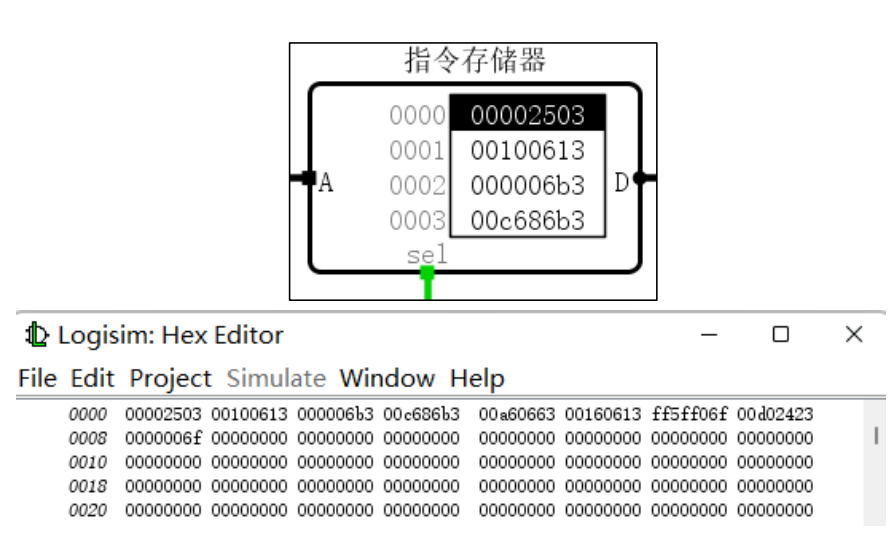
\includegraphics[width=0.8\textwidth]{3.5.1.png}
        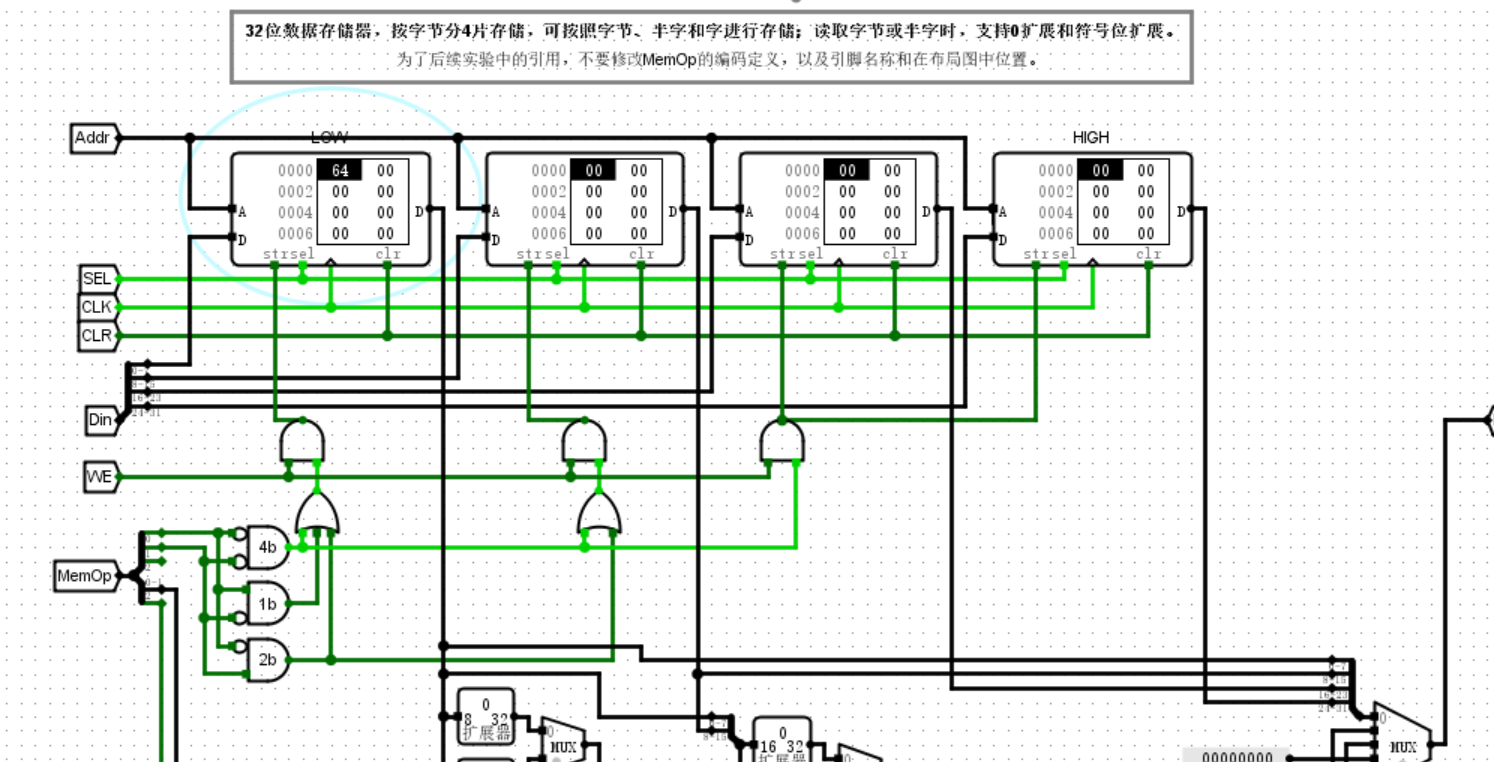
\includegraphics[width=0.8\textwidth]{3.5.2.png}
        \caption{累加和程序数据导入图}
    \end{figure}
    \begin{figure}[H]
        \centering
        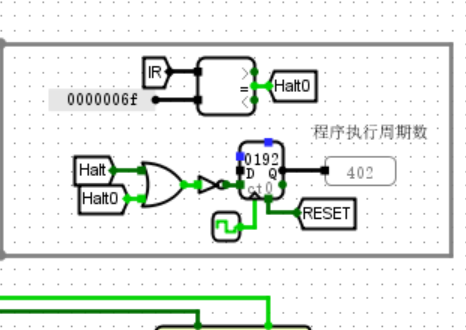
\includegraphics[width=0.8\textwidth]{3.5.3.png}
        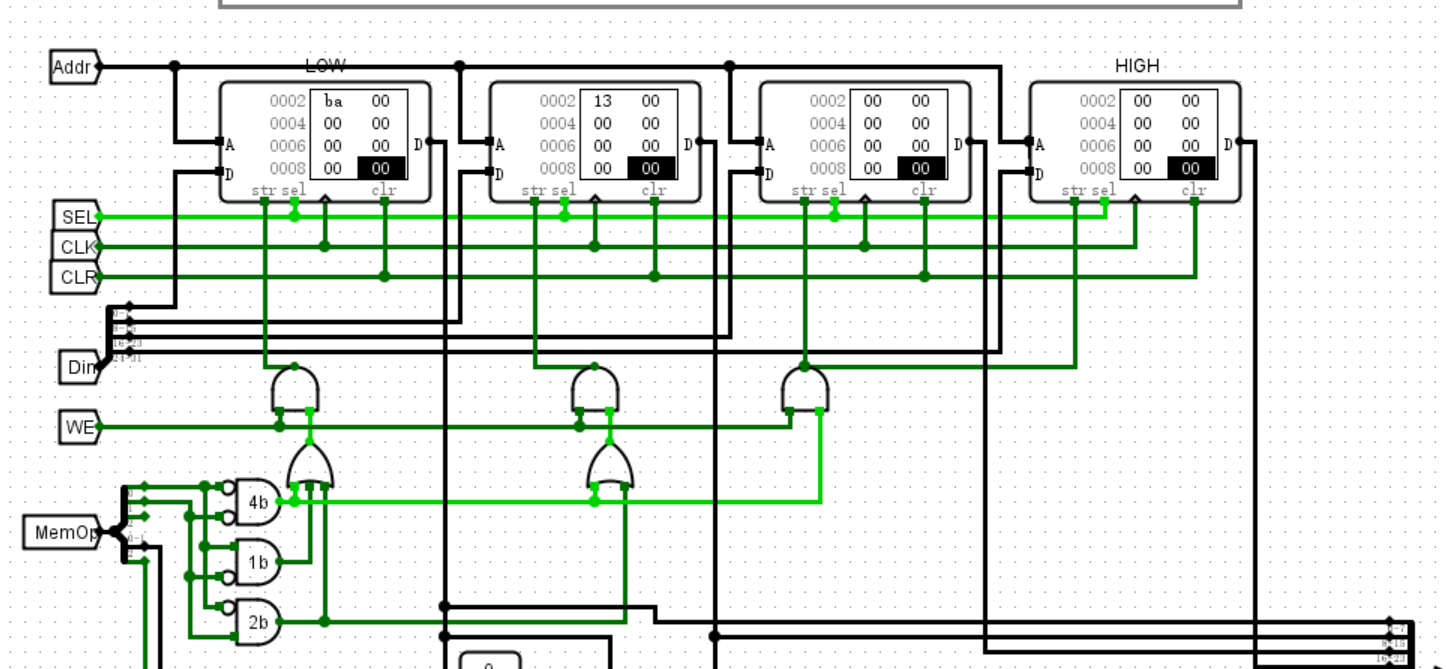
\includegraphics[width=0.8\textwidth]{3.5.4.png}
        \caption{累加和程序数据验证图}
    \end{figure}
    可以看到运行了402个周期,最终累加和的计算机结果为 0x13ba(十进制数 5050),与预期结果一致。

    \subsection{用冒泡排序程序进行 CPU 设计验证}

    汇编代码中将数据个数 $n$ 读到寄存器 $a0$,常量 $1$ 保存在寄存器 $a1$ 中,外循环变量 $i$ 保存在 $a2$,内循环变量 $j$ 保存在 $a3$,第 $j$ 个元素 $a[j]$的地址存放 $a4$。第 $j$ 个元素 $a[j]$读入 $a6$,第 $j+1 $个元素 $a[j+1]$读入 $a7$。\par
    在指令存储器中加载冒泡程序可执行机器代码数据镜像文件bubble.hex,打开数据存储器子电路,在最低字节 RAM 中加载待排序数据镜像文件bubble.dat,观察运行情况。

    \subsubsection{仿真测试图}

    \begin{figure}[H]
        \centering
        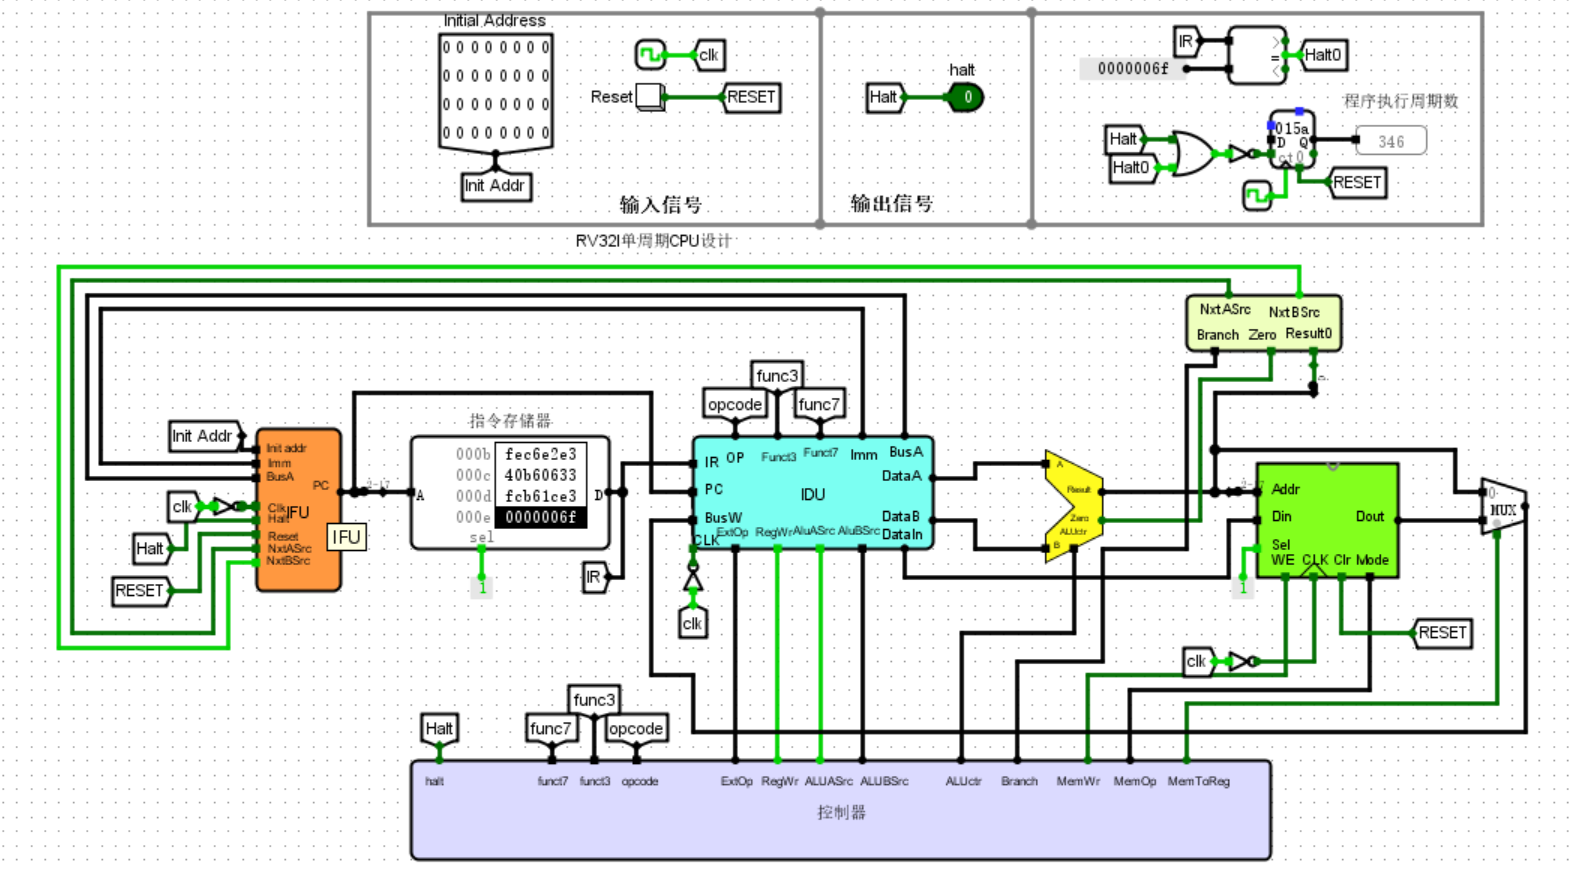
\includegraphics[width=0.8\textwidth]{4.5.1.png}
        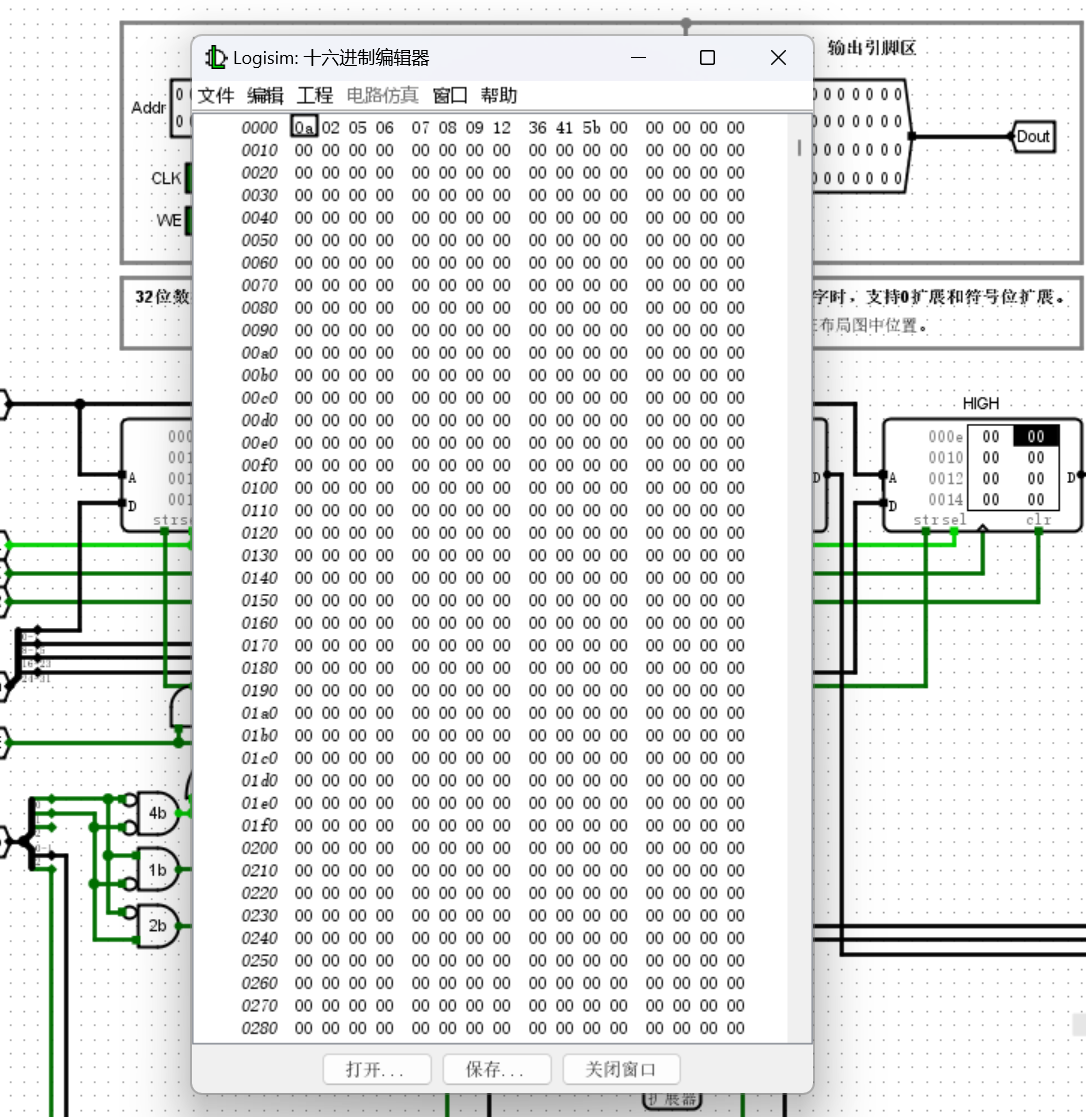
\includegraphics[width=0.8\textwidth]{4.5.2.png}
        \caption{累加和程序数据验证图}
    \end{figure}
    打开最低字节 RAM,可以看到数据已经被排序:a 2 5 6 7 8 9 12 36 41 5b

    \subsection{C程序汇编测试}
    将 b-sort-riscv32-npc.bin-logisim-inst.txt 文件加载到指令存储器中,将b-sort-riscv32-npc.bin-logisim-data0.txt 加载到最低字节的数据存储器中,将 b-sort-riscv32-npc.bin-logisim-data1.txt 加载到次低字节的数据存储器,以此类推,加载 b-sort-riscv32-npc.bin-logisim-data2.txt、b-sort-riscv32-npc.bin-logisim-data3.txt 到指定的数据存储器中。选择连续时钟信号,启动程序,分析程序执行的结果。
    \begin{figure}[H]
        \centering
        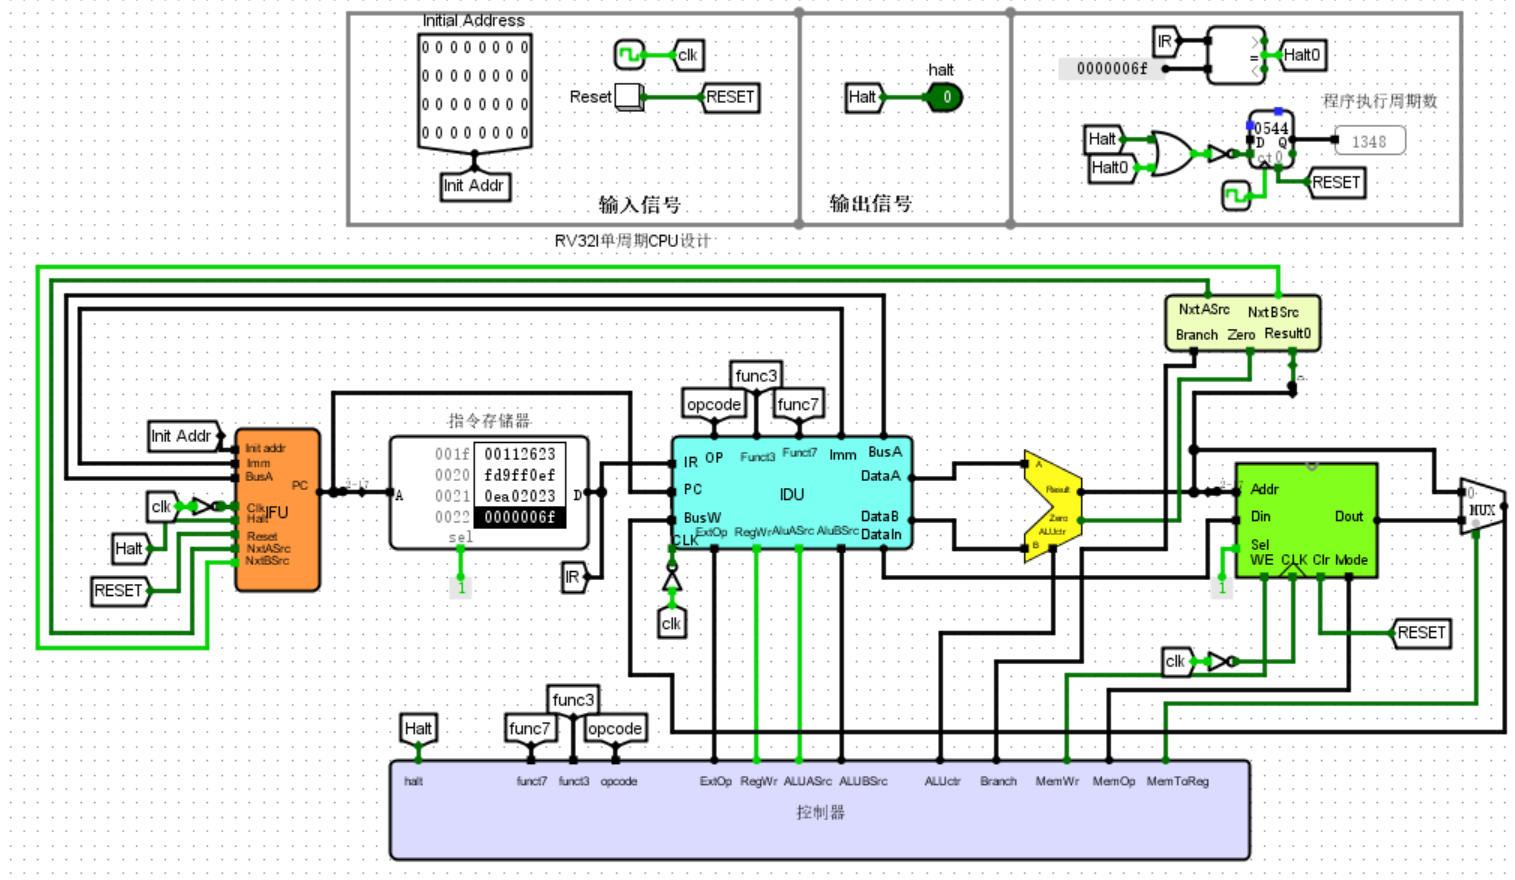
\includegraphics[width=0.8\textwidth]{5.5.1.png}
        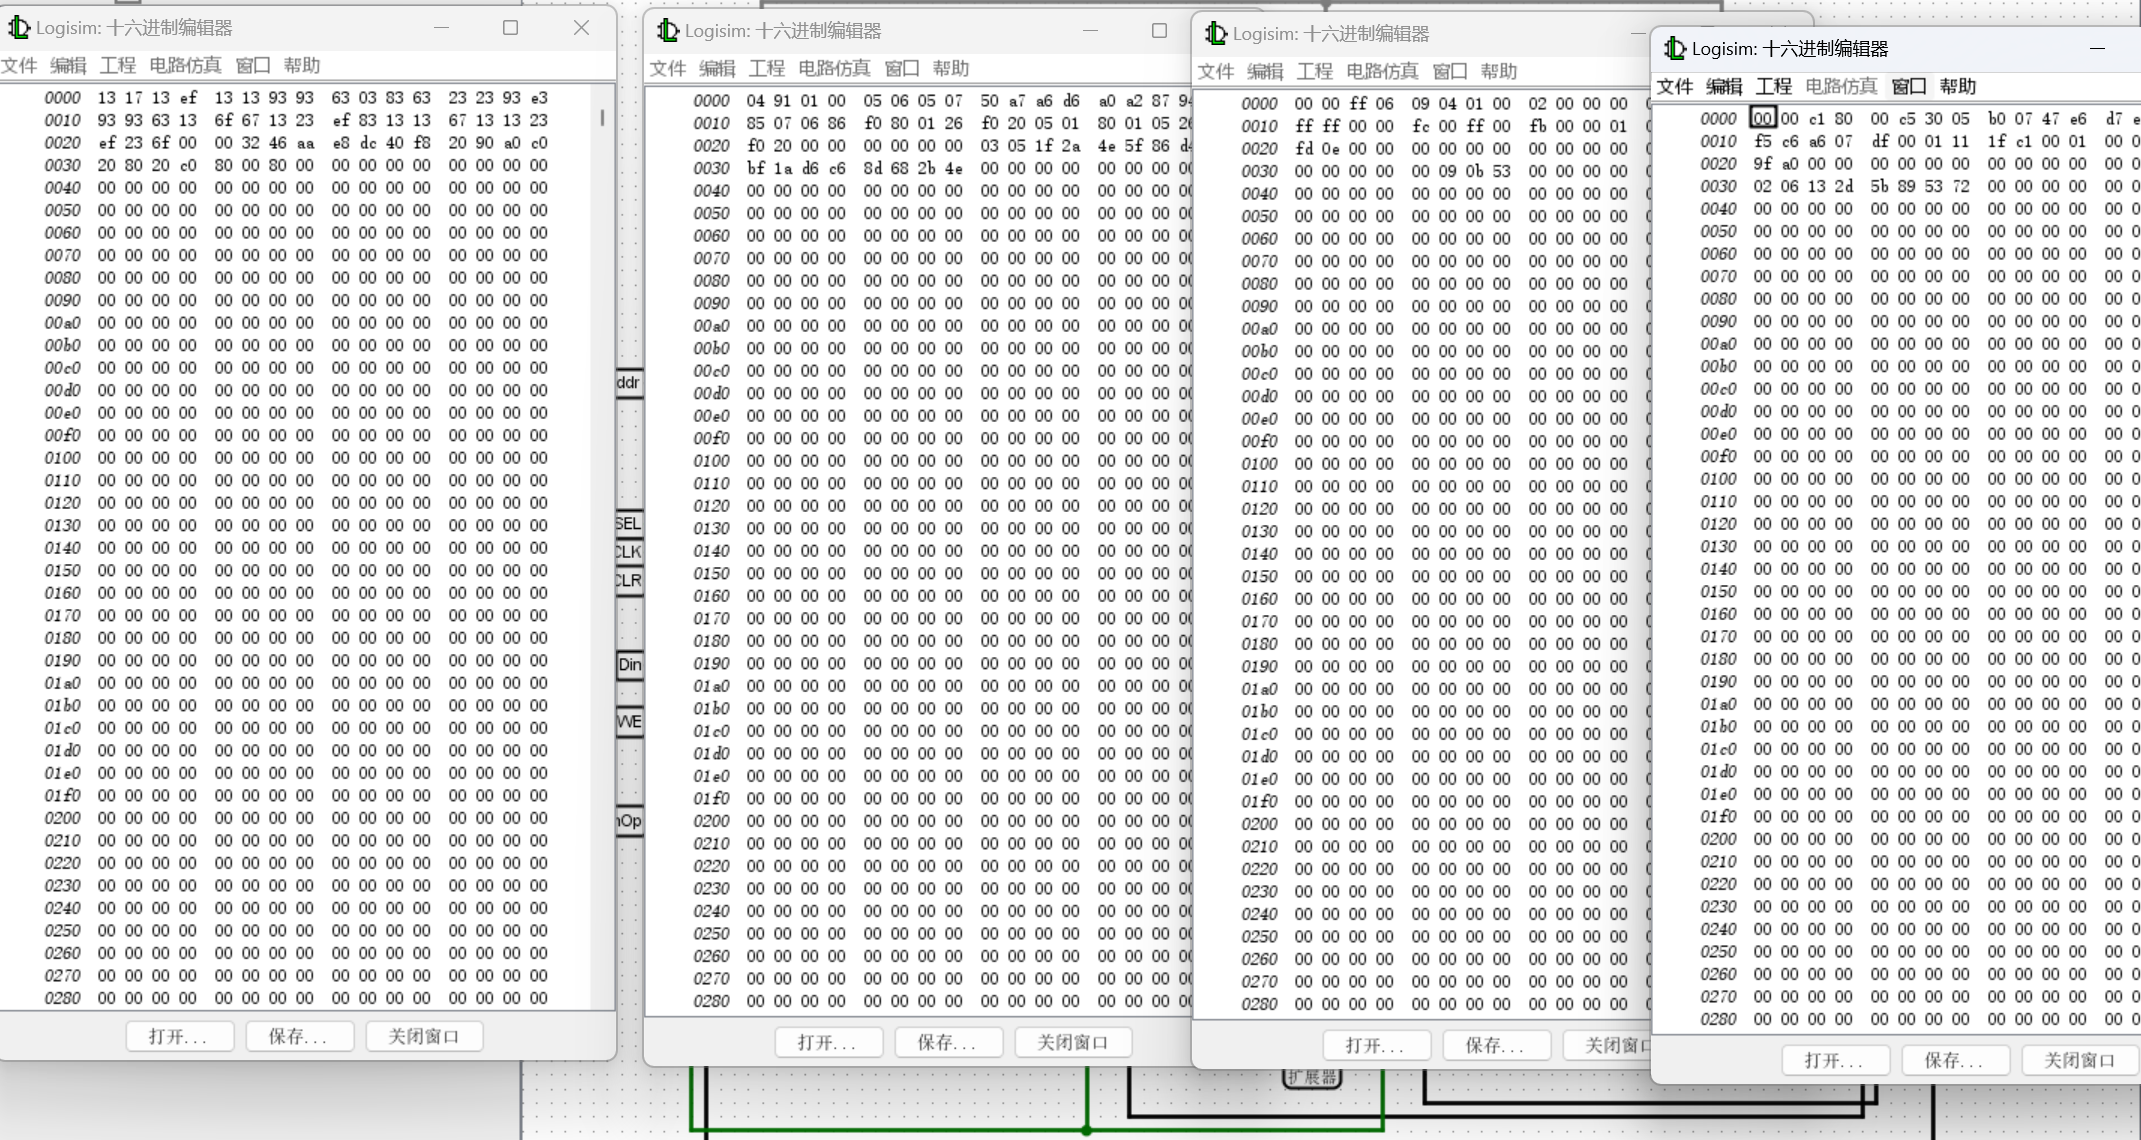
\includegraphics[width=0.8\textwidth]{5.5.2.png}
        \caption{C程序验证图}
    \end{figure}
    程序运行了1348个周期,最终排序结果经整理如下,符合预期。、
    \begin{figure}[H]
        \centering
        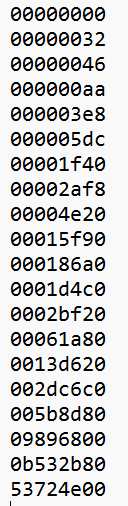
\includegraphics[width=0.4\textwidth]{5.5.3.png}
    \caption{C程序验证结果}
    \end{figure}

    \section{思考题}


    \subsection{在累加和计算程序中,添加溢出判读语句,并把最大的不溢出累计和以及累加序数保存到数据存储器中输出。}
    在累加和计算程序中,添加溢出判断语句可以在每次累加操作后进行。可以通过比较累加结果和数据存储器中的最大值来判断是否发生了溢出。如果发生了溢出,需要将累加序数和最大不溢出累计和保存到数据存储器中输出。\\
    可以在累加指令"add a3, a3, a2"之后添加如下代码:
    \begin{lstlisting}[language=C]
    addiw a4, a3, 0 # 将累加和 a3 的低 32 位复制到 a4 中
    blt a4, a3, overflow # 若 a4 < a3,则说明溢出,跳转到 overflow 处
    j continue # 若未溢出,则跳转到 continue 处
    \end{lstlisting}
    在溢出处理代码"overflow"处,可以将最大不溢出的累计和以及累加序数保存到数据存储器中输出。具体来说,可以添加如下代码:
    \begin{lstlisting}[language=C]
    sub a5, a5, a0 # 减去最后一个元素的值
    sw a5, 4(x0) # 将最大不溢出的累计和保存到数据存储器 0x0004 单元
    addi a6, a2, -1 # 将累加序数设为 i-1
    sw a6, 12(x0) # 将累加序数保存到数据存储器 0x000C 单元
    j end # 跳转到程序结束处
    \end{lstlisting}
    完整的代码如下:
    \begin{lstlisting}[language=C]
    main:
    lw a0,0(x0) # 从数据存储器地址 0x0000 单元中读取参数 n 到寄存器 a0;
    addi a2, x0,1 # 循环变量 i,存放在 a2,初值为 1
    add a3,x0,x0 # 累计和存放在 a3,初值为 0
    loop:
    add a3, a3, a2 # 将 a3=a3+i
    addiw a4, a3, 0 # 将累加和 a3 的低 32 位复制到 a4 中
    blt a4, a3, overflow # 若 a4 < a3,则说明溢出,跳转到 overflow 处
    j continue # 若未溢出,则跳转到 continue 处
    overflow:
    sub a5, a5, a0 # 减去最后一个元素的值
    sw a5, 4(x0) # 将最大不溢出的累计和保存到数据存储器 0x0004 单元
    addi a6, a2, -1 # 将累加序数设为 i-1
    sw a6, 12(x0) # 将累加序数保存到数据存储器 0x000C 单元
    j end # 跳转到程序结束处
    continue:
    beq a2, a0, finish # 若 i=n,则跳出循环
    addi a2, a2, 1 # i++
    jal x0, loop # 无条件跳转到 loop 执行
    finish:
    sw a3, 8(x0) # 将累加结果保存到数据存储器 0x0008 单元
    end:
    jal x0, end # 无条件跳转到 end
    \end{lstlisting}

    \subsection{如果分支跳转指令不在 ALU 内部使用减法运算来实现,而是在 ALU 外使用独立比较器来实现,说说单周期 CPU 的电路原理图中需要做哪些修改?}
    \begin{enumerate}
        \item 修改控制逻辑:将分支跳转指令的识别和控制信号生成从 ALU 控制部分移动到比较器模块控制部分。
        \item 修改指令解码器:将分支跳转指令的识别从 ALU 操作码识别部分移动到比较器操作码识别部分。
        \item 修改DataPath:将比较器的输出和控制信号传递到 PC 寄存器和数据存储器,以实现分支跳转指令的功能。
    \end{enumerate}



    \subsection{实现单周期 CPU 后,如何实现键盘输入、TTY 输出部件等输入输出设备的数据访问,构建完整的计算机系统。}
    \begin{enumerate}
        \item 键盘输入:可以通过添加一个键盘控制器,将键盘输入数据传输到CPU中。键盘控制器可以使用PS/2或USB接口与键盘连接,并将输入数据传输到CPU的I/O地址空间。CPU可以通过读取I/O地址空间来获取键盘输入数据。
        \item TTY输出:可以通过添加一个串行通信控制器,将CPU输出数据传输到TTY设备中。串行通信控制器可以使用RS-232或USB接口与TTY设备连接,并将输出数据转换为串行数据流进行传输。CPU可以通过写入I/O地址空间来将输出数据传输到串行通信控制器中。
    \end{enumerate}


    \subsection{如果需要实现 5 级流水线 RV32I CPU,则如何在单周期 CPU 基础上进行修改?}
    \begin{enumerate}
        \item 增加流水线寄存器:在单周期CPU的基础上,需要增加5个流水线寄存器,用于保存不同阶段的指令执行结果。这些寄存器可以用D触发器实现。
        \item 增加控制逻辑:需要增加控制逻辑,用于控制流水线的各个阶段。
        \item 增加数据冲突检测。
        \item 增加分支预测。
    \end{enumerate}
    

\end{document}